\documentclass[tombow,dvipdfmx]{corona-a5-1.1}
% dvipdfmxを追加(川口)

% Springer document settings
\usepackage[bottom]{footmisc}% places footnotes at page bottom

\usepackage{newtxtext}       % 
\usepackage[varvw]{newtxmath}       % selects Times Roman as basic font
%%%%%%%%%%%%%%%%%%%%%%%%%%%%%%%

% \usepackage{amssymb}
\usepackage{ntheorem}
\usepackage{amsmath}
\usepackage{enumitem}


\usepackage{graphicx}
\usepackage{color}
\usepackage{cite}
\usepackage{makeidx}


\usepackage{ascmac}
\usepackage{eclbkbox}
\usepackage{dsfont}

\usepackage{longtable}

\usepackage{url}

\usepackage{hyperref}

\usepackage{multicol}

%% --川口追加--
\makeatletter
\let\MYcaption\@makecaption
\makeatother
\usepackage{subcaption}
\captionsetup{compatibility=false}      % 必要に応じて

\makeatletter
\let\@makecaption\MYcaption
\makeatother
% ----

%%
\theoremstyle{plain}
\theoremheaderfont{\bfseries}
\theorembodyfont{\rmfamily}
\theoremseparator{\hspace{1ex}}
\theoremindent0cm
\theoremnumbering{arabic}
\theoremprework{\vspace{1ex}\begin{shadebox}\vspace{1ex}}
\theorempostwork{\vspace{-1ex}\end{shadebox}\vspace{1ex}}

%%
\theoremclass{theorem}

%%
\theoremclass{theorem}

%%
\theoremclass{theorem}


%%
\theoremstyle{break}
\theoremheaderfont{\bfseries}
\theorembodyfont{\rmfamily}
\theoremseparator{}
\theoremindent0cm
\theoremnumbering{arabic}
\theoremprework{\vspace{1.5ex}\begin{breakbox}\vspace{-0.5ex}}
\theorempostwork{\vspace{-0.5ex}\end{breakbox}\vspace{1.5ex}}

%%
\theoremstyle{nonumberplain}
\theoremseparator{\hspace{1ex}}

%%
\newtheorem{assumption}{Assumption}[section]

%%
\renewcommand{\theproblem}{}

\renewcommand{\theremark}{}


\newcommand{\red}[1]{{\color{red}#1}}
\newcommand{\blue}[1]{{\color{blue}#1}}
\newcommand{\green}[1]{{\color{green}#1}}

\DeclareMathOperator*{\argmax}{arg\,max}

\newcommand{\bm}[1]{\boldsymbol{#1}}
\newcommand{\sfT}{\mathsf{T}}

\newcommand{\advanced}{$^{\ddag}$}

\DeclareMathOperator{\sfsin}{\mathsf{sin}}
\DeclareMathOperator{\sfcos}{\mathsf{cos}}
\DeclareMathOperator{\sftan}{\mathsf{tan}}
\DeclareMathOperator{\sfarctan}{\mathsf{arctan}}

\DeclareMathOperator{\sfdiag}{\mathsf{diag}}
\DeclareMathOperator{\sfcol}{\mathsf{col}}
\DeclareMathOperator{\sfdet}{\mathsf{det}}
\DeclareMathOperator{\sfadj}{\mathsf{adj}}
\DeclareMathOperator{\sftrace}{\mathsf{trace}}

\DeclareMathOperator{\real}{\mathsf{Re}}

\DeclareMathOperator{\sfker}{\mathsf{ker}}
\DeclareMathOperator{\sfim}{\mathsf{im}}

\DeclareMathOperator{\sfdim}{\mathsf{dim}}
\DeclareMathOperator{\sfspan}{\mathsf{span}}

\DeclareMathOperator{\sfint}{\mathsf{int}}

\DeclareMathOperator*{\sfmin}{\mathsf{min}}
\DeclareMathOperator*{\sfmax}{\mathsf{max}}
\DeclareMathOperator*{\sfsup}{\mathsf{sup}}

\DeclareMathOperator{\sfsat}{\mathsf{sat}}

\newcommand{\mat}[1]{\left[\: \begin{matrix} #1 \end{matrix} \:\right]}
\newcommand{\spliteq}[1]{\begin{split} #1 \end{split}}
\newcommand{\simode}[1]{\begin{cases}  \begin{split} #1 \end{split} \end{cases}}

\newcommand{\proofend}{\hfill \rule{2mm}{3mm}}

\newcommand{\Xti}{X_i'}
\newcommand{\Xsi}{X_i}

\newcommand{\Xtone}{X_1'}
\newcommand{\XtN}{X_N'}

\newcommand{\Xt}{X'}
\newcommand{\Xs}{X}

\newcommand{\taudi}{\tau_i}
\newcommand{\taud}{\tau}

\newcommand{\Cgi}{b_i}


\newcommand{\Ifd}{I_{\rm field} }

\newcommand{\matlab}{\textsc{Matlab} }





%% --川口追加--
\newcommand{\thshift}{\theta_{12}}
\newcommand{\thshiftb}{\theta_{32}}
\newcommand{\Ysa}{\bm y_{12}}
\newcommand{\bca}{c_{12}}
\newcommand{\Ysb}{\bm y_{32}}
\newcommand{\bcb}{c_{32}}
\newcommand{\bcij}{c_{ij}}
\newcommand{\Is}{{\bm I}_{12}' }
\newcommand{\im}{\bm j}
\newcommand{\tr}{{\sf T}}

%%%%%%%%%%%%%%%%%%%%%%%%% code lines %%%%%%%%%%%%%%%%%%%%%%%%%%%%%%%%%%%%%%%%%%
\usepackage{listings}
\usepackage{xcolor}
\renewcommand{\lstlistingname}{Program}% Listing -> Algorithm
\renewcommand{\lstlistlistingname}{List of \lstlistingname s}% List of Listings -> List of Algorithms

\definecolor{codegreen}{rgb}{0,0.6,0}
\definecolor{codegray}{rgb}{0.5,0.5,0.5}
\definecolor{codepurple}{rgb}{0.58,0,0.82}
\definecolor{backcolour}{rgb}{0.95,0.95,0.92}

\lstdefinestyle{mystyle}{
    backgroundcolor=\color{backcolour},   
    commentstyle=\color{codegreen},
    keywordstyle=\color{magenta},
    numberstyle=\tiny\color{codegray},
    stringstyle=\color{codepurple},
    basicstyle=\ttfamily\footnotesize,
    breakatwhitespace=false,         
    breaklines=true,                 
    captionpos=b,                    
    keepspaces=true,                 
    numbers=left,                    
    numbersep=5pt,                  
    showspaces=false,                
    showstringspaces=false,
    showtabs=false,                  
    tabsize=2
}

\lstset{style=mystyle}


\begin{document}
\chapter{電力系統モデルの数値シミュレーション}\label{chap:numcal}

チャプター概要

\section{電力系統モデルの時間応答を計算するためには}\label{sec:howtocal}
\subsection{潮流計算の実装法}
%{
\newcommand{\omitcode}{~(略)~}
\newcommand{\tr}{{\sf T}}
MATLABを用いて潮流計算を行うプログラムを実装する方法について説明する。
潮流計算のためには,式\ref{eq:ohmY2}の連立方程式を解く必要がある。
そこで,まずは電力システムではない簡単な例題を用いて,連立方程式をMATLABで解く方法を示す。
\begin{例}[簡単な例題]\label{ex:algenraic_equation_ex1}
代数方程式
\begin{subequations}\label{eq:algebraic_equation_ex1}
\begin{align}
x^2 - y = 0\\
x^2 + y^2 - 2 = 0
\end{align}
\end{subequations}
を満たす$(x, y)$の組を数値計算によって求めることを考える。
ここで,この解は$(x, y) = (-1, 1),\ (1, 1)$の2つであることに注意しよう。
MATLABで代数方程式を解くためには,\verb{optimization toolbox}の\verb{fsolve}
コマンドが便利である。このコマンドを用いるためには,代数方程式$f(x)=0$の$f(x)$にあたる部分,
すなわち,式(\ref{eq:algebraic_equation_ex1})の左辺を評価する関数を実装する必要がある。
この関数を\verb{func\_ex1.m}という名前のファイルとして実装すると,
プログラム\nobreak\ref{program:ex1}のようになる。

\begin{PROGRAMA}[count,title={func\_ex1.m}]\label{program:ex1}
\begin{verbatim}
function out = func_ex1(x_in)

x = x_in(1);
y = x_in(2);

out = zeros(2, 1);
out(1) = x^2 - y;
out(2) = x^2 + y^2 - 2;

end
\end{verbatim}
\end{PROGRAMA}

つぎに,この関数を用いて\verb{fsolve}を実行し,代数方程式を解くプログラムを記述すると,
プログラム\nobreak\ref{program:ex1_main}となる。
\begin{PROGRAMA}[count,title={main\_ex1.m}]\label{program:ex1_main}
\begin{verbatim}
options = optimoptions('fsolve', 'Display', 'iter');
x0 = [0.1; 0.5];
x_sol = fsolve(@func_ex1, x0, options)
\end{verbatim}
\end{PROGRAMA}

ここで,\verb{options}は最適化を行うときのオプションを設定しており,
この例では最適化の過程を画面に表示することを示している。また,
\verb{x0 = [0.1; 0.5];}は数値計算によって最適化を行う際の初期値を表している。
このプログラムを実行すると,つぎの実行結果が得られる。

\begin{実行結果}
\begin{verbatim}
  Iteration  Func-count     f(x)     (略)
      0          3          3.2677
      1          6        0.282554
\end{verbatim}
\omitcode
\begin{verbatim}
      4         15     3.60447e-14

  方程式が解かれました。
\end{verbatim}
\omitcode
\begin{verbatim}
  x_sol =
      1.0000
      1.0000
\end{verbatim}
\end{実行結果}

この実行結果から,反復を行うにつれて$f(x)$の値が小さくなり,
最終的に$f(x)\approx 0$となる解が見つかっていることがわかる。
このとき見つかった解は$(x, y) = (1, 1)$であり,これは実際に連立方程式の解である。
ここで,\verb{fsolve}を用いた数値解法では,すべての
解が得られるわけではなく,解のうちのどれか
一つが得られるに過ぎないことに注意しよう。
もう一つの解が得られる場合を示すために,
プログラム\nobreak\ref{program:ex1_main}の2行目を
\verb{x0 = [-0.1; 0.5];}
と変更した場合の結果をつぎに示す。

\begin{実行結果}
\begin{verbatim}
    Iteration  Func-count     f(x)     (略)
        0          3          3.2677
        1          6        0.282554
\end{verbatim}
\omitcode
\begin{verbatim}
        4         15     3.60447e-14
   
   方程式が解かれました。
\end{verbatim}
\omitcode
\begin{verbatim}
   x_sol =
   
      -1.0000
       1.0000
\end{verbatim}
\end{実行結果}

この結果では,もう一つの解$(x, y) = (-1, 1)$が得られていることがわかる。
このように,数値解法を用いる非凸な最適化では,初期値によって異なる解が得られることに注意が必要である。
つぎに,プログラム\nobreak\ref{program:ex1_main}の2行目を
\verb{x0 = [-0.1; -0.1];}
とした場合の実行結果を見てみよう。

\begin{実行結果}
    \begin{verbatim}
        Iteration  Func-count     f(x)     (略)
        0          3          3.2877
        1          6          2.4674
\end{verbatim}
    \omitcode
    \begin{verbatim}
       33         74            1.75       

       解が見つかりませんでした。
    \end{verbatim}
    \omitcode
    \begin{verbatim}
        x_sol =

        -0.0000
        -1.2247
    \end{verbatim}
\end{実行結果}

この例からわかるように初期値の与え方によっては実際には解が存在する方程式であっても
解が得られないこともあり得る。実用上は求めたい解に近い初期値を与えることが重要である。
\end{例}

つぎに,潮流計算を行うプログラムの単純な実装法について紹介する。
\begin{例}[潮流計算の解き方]\label{ex:simplepowerflow}
図\ref{dummy}の電力システムに対する潮流計算を行うことを考える。
潮流計算も代数方程式を解く計算の一種であるため,
例\nobreak\ref{ex:algenraic_equation_ex1}と同様に,$f(x)=0$の
$f(x)$の部分を実装することが必要である。
ここでは,
送電線のパラメータ$(\bm y_{12}, \bm y_{23})=(1.3652-11.6030\bm j, -10.5107 \bm j)$が与えられたもとで,
\ref{tab:datasheet_ex2}のデータシートに整合する
潮流状態
\[
\bigl(
|\bm{I}_1(t)|,\angle \bm{I}_1(t),
|\bm{V}_1(t)|,\angle \bm{V}_1(t),
\ldots
|\bm{I}_3(t)|,\angle \bm{I}_3(t),
|\bm{V}_3(t)|,\angle \bm{V}_3(t)
\bigr)
\]
を決定することを考える。
\begin{table}[htb]
    \centering
     \caption{潮流計算のためのデータシート}\label{tab:datasheet_ex2}
      \begin{tabular}{cccccc}
        $i$ & 種類 & $|\bm V_i|$ & $\angle \bm V_i$ & $P_i$ & $Q_i$\\\hline\hline
        1 & スラック & 2 & 0 & - & -\\
        2 & 負荷 & - & - & $-3$ & 0 \\
        3 & 発電機 & 2 & - & 0.5  & - \\
        \hline
      \end{tabular}
\end{table}
送電線のパラメータから構成されるアドミタンス行列$\bm Y$が与えられると,電流は電圧に依存して
一意に定まるため,潮流計算は実質的には電圧の組を決める手続きとなる。
このことから,代数方程式における変数$x$は,電圧フェーザの組を表せば良いことがわかる。
ここでは,電圧フェーザの実部と虚部を並べて$x$とすることにする
\footnote{もちろん,電圧フェーザの絶対値と偏角の組を$x$としたプログラムも同様に書ける}。

変数$x$から電圧フェーザ$\bm V=[\bm V_1, \bm V_2, \bm V_3]^\tr$を構成すると,
\[
\bm I = \bm Y \bm V    
\]
によって電流フェーザの組$\bm I=[\bm I_1, \bm I_2, \bm I_3]^\tr$
が定まる。この$\bm I$と$\bm V$を使えば,各母線の
有効電力$P$と無効電力$Q$を計算することができる。
すなわち,電圧,電流,有効電力,無効電力の組が$x$の関数として表せることになる。
これを$\hat{\bm V}_i(x)$,$\hat{\bm I}_i(x)$,$\hat{P}_i(x)$,$\hat{Q}_i(x)$と
すると,解くべき連立方程式は
\begin{align*}
    |\bm V_1|-|\hat{\bm V}_1(x)| &= 0\\
    \angle \bm V_1 - \angle \hat{\bm V}_1(x) &= 0\\
    P_2 -\hat P_2(x) &= 0\\
    Q_2 -\hat Q_2(x) &= 0\\
    P_3 -\hat P_3(x) &= 0\\
    |\bm V_3|-|\hat{\bm V}_3(x)| &= 0
 \end{align*}
 である。この左辺を愚直に実装すると,
 プログラム\nobreak\ref{program:ex2}のようになる\footnote{この関数は5つの出力引数を持つが,
 \verb{fsolve}では1つ目の出力引数のみが用いられる。残りの引数は結果の確認のために追加したものである。}。
\begin{PROGRAMA}[count, title={func\_ex2.m}]\label{program:ex2}
\begin{verbatim}
function [out, Vhat, Ihat, Phat, Qhat] = func_ex2(x)
% x: [Real(V1), Imag(V1),
%     Real(V2), Imag(V2),
%     Real(V3), Imag(V3)]';

% 送電線
y12 = 1.3652 - 11.6040j;
y23 = -10.5107j;
Y = [y12, -y12, 0;
    -y12, y12+y23, -y23;
    0, -y23, y23];

% スラック母線
V1abs = 2;
V1angle = 0;

% 負荷母線
P2 = -3;
Q2 = 0;

% 発電機母線
P3 = 0.5;
V3abs = 2;

V1hat = x(1) + 1j*x(2);
V2hat = x(3) + 1j*x(4);
V3hat = x(5) + 1j*x(6);

Vhat = [V1hat; V2hat; V3hat];

Ihat = Y*Vhat;
PQhat = Vhat.*conj(Ihat);
Phat = real(PQhat);
Qhat = imag(PQhat);

out = [V1abs-abs(V1hat); V1angle-angle(V1hat);
    P2-Phat(2); Q2-Qhat(2);
    P3-Phat(3); V3abs-abs(V3hat)];
end
\end{verbatim}
\end{PROGRAMA}

例\nobreak\ref{ex:algenraic_equation_ex1}で見たように,
代数方程式を解くときには初期値の設定が重要である。
潮流計算でよく用いられる初期値の1つに\textcolor{red}{フラットスタート(?)}
と呼ばれるものがある。フラットスタートでは,$|\hat{\bm V}_i(x)|=1$,$\angle \bm V_i(x) = 0$
となるように$x$の初期値を決める。これを用いて潮流計算を解くプログラムは
プログラム\nobreak\ref{program:ex2_main}のようになる。
\begin{PROGRAMA}[count,title={main\_ex2.m}]\label{program:ex2_main}
\begin{verbatim}
x0 = [1; 0; 1; 0; 1; 0];
options = optimoptions('fsolve', 'Display', 'iter');
x_sol = fsolve(@func_ex2, x0, options);
[~, V, I, P, Q] = func_ex2(x_sol);
Vabs = abs(V);
Vangle = angle(V);
display('Vabs:'), display(Vabs')
display('Vangle:'), display(Vangle')
display('P:'), display(P')
display('Q:'), display(Q')
\end{verbatim}
\end{PROGRAMA}

このプログラムを実行した結果の例はつぎのようになり,
結果として,\ref{tab:result_ex2}の結果が得られる。
この結果は\ref{tab:datasheet_ex2}の制約と整合するものである。

\begin{実行結果}
\begin{verbatim}
 Iteration  Func-count     f(x)     (略)
     0          7           11.25 
     1         14         3.28327 
\end{verbatim}
\omitcode
\begin{verbatim}
     5         42     4.19428e-28

方程式が解かれました。
\end{verbatim}
\omitcode
\begin{verbatim}
Vabs:
    2.0000    1.9918    2.0000

Vangle:
    0.0000   -0.0538   -0.0419

P:
    2.5158   -3.0000    0.5000

Q:
   -0.0347    0.0000    0.1759
\end{verbatim}
\end{実行結果}
\begin{table}
\centering
\caption{潮流計算の結果}\label{tab:result_ex2}
 \begin{tabular}{cccccc}
   $i$ & 種類 & $|\bm V_i|$ & $\angle \bm V_i$ & $P_i$ & $Q_i$\\\hline\hline
   1 & スラック & 2 & 0 & 2.5158 & -0.0347\\
   2 & 負荷 & 1.9918 & -0.0538 & $-3$ & 0 \\
   3 & 発電機 & 2 & -0.0419 & 0.5  & 0.1759\\
\hline
 \end{tabular}
\end{table}
\end{例}

% \begin{COLUMN}
% 例\nobreak\ref{ex:algenraic_equation_ex2}
% % のプログラムでは,各種のパラメータは\verb{func_ex2.m}の中で
% % 定義されている。様々な条件での潮流計算を行うことを考えて,
% % \verb{main_ex2.m}のファイルにパラメータを記述したくなることがある。
% % グローバル変数はあかん。
% \end{COLUMN}

\begin{例}[より良い実装]
\ref{ex:simplepowerflow}で潮流計算の実装法について述べた。
この実装では,ネットワークの構成が代わるたびにプログラム\ref{program:ex2}に相当する関数を書き換える必要がある。
このような書き換えを最小限にするために,プログラムを
モジュール群に分割し,構造化して見透し良く実装する方法について述べる。

まず,関数のなかでアドミタンス行列を作成している部分を分離しよう。
このためには変数\verb{Y}を関数の入力引数に移せば良い。
このときのコードは\label{program:ex3}のようになる。
\begin{PROGRAMA}[count, title={func\_ex3.m}]\label{program:ex3}
\begin{verbatim}
function [out, Vhat, Ihat, Phat, Qhat] = func_ex2(x, Y)
% スラック母線
V1abs = 2;
V1angle = 0;
(略)
out = [V1abs-abs(V1hat); V1angle-angle(V1hat);
    P2-Phat(2); Q2-Qhat(2);
    P3-Phat(3); V3abs-abs(V3hat)];
end
\end{verbatim}
\end{PROGRAMA}

しかしながら,\verb{fsolve}は最適化するパラメータを
唯一の引数とする関数を要求するため,この関数を直接用いることはできない。
この問題は関数のカリー化という技術を用いることで解決することができる。
カリー化を行って\verb{fsolve}を適用するプログラムは\ref{program:ex3_main}のようになる。
\begin{PROGRAMA}[count,title={main\_ex3.m}]\label{program:ex3_main}
\begin{verbatim}
x0 = [1; 0; 1; 0; 1; 0];
options = optimoptions('fsolve', 'Display', 'iter');
y12 = 1.3652 - 11.6040j;
y23 = -10.5107j;
Y = [y12, -y12, 0;
    -y12, y12+y23, -y23;
    0, -y23, y23];
func_curried = @(x) func_ex3(x, Y);

x_sol = fsolve(func_curried, x0, options);
(略)
\end{verbatim}
\end{PROGRAMA}
このプログラムの8行目において,
2つの入力引数のうち,1つの引数のみを残した新たな関数を
生成している。
このような方法をカリー化と呼び,
これを用いると,グローバル変数を用いることなく
機能の分離を行うことができる。

つぎに,それぞれの母線における制約条件を計算する
プログラムを考える。プログラム\ref{program:ex2}は,
それぞれの母線の制約条件がハードコーディングされていることの他に,
母線の種類による場合分けが暗に含まれているという問題点を抱えている。
このような実装では,
母線の種類が増えたときには,場合分けの処理を書き直す必要がある。

この場合分けを避けた記述を行うためには,
オブジェクト指向の考え方を用いると便利である。
まず,スラック母線,発電機母線,負荷母線に対応するクラスを定義し,
そのインスタンスを活用することにする。
このとき,それぞれの種類の母線では異なる制約条件が設定されるが,
「制約条件をもつ」という点では共通である。
この共通の性質は,共通の名前をもつメソッドとして実装されるべきである。
この考え方を用いた実装はプログラム\ref{program:bus_slack}--\ref{program:ex4}となる。

\begin{PROGRAMA}[count,title={bus\_slack.m}]\label{program:bus_slack}
\begin{verbatim}
classdef bus_slack

properties
    Vabs
    Vangle
end

methods
    function obj = bus_slack(Vabs, Vangle)
        obj.Vabs = Vabs;
        obj.Vangle = Vangle;
    end
    
    function out = get_constraint(obj, Vr, Vi, P, Q)
        Vabs = norm([Vr; Vi]);
        Vangle = atan2(Vi, Vr);
        out = [Vabs-obj.Vabs; Vangle-obj.Vangle];
    end
end
end
\end{verbatim}
\end{PROGRAMA}

\begin{PROGRAMA}[count,title={bus\_PV.m}]\label{program:bus_PV}
\begin{verbatim}
classdef bus_PV

properties
    P
    Vabs
end

methods
    function obj = bus_PV(P, Vabs)
        obj.P = P;
        obj.Vabs = Vabs;
    end
    
    function out = get_constraint(obj, Vr, Vi, P, Q)
        Vabs = norm([Vr; Vi]);
        out = [obj.P-P; Vabs-obj.Vabs];
    end
end
end
\end{verbatim}
\end{PROGRAMA}

\begin{PROGRAMA}[count,title={bus\_PQ.m}]\label{program:bus_PQ}
\begin{verbatim}
classdef bus_PQ

properties
    P
    Q
end

methods
    function obj = bus_PQ(P, Q)
        obj.P = P;
        obj.Q = Q;
    end
    
    function out = get_constraint(obj, Vr, Vi, P, Q)
        out = [P-obj.P; Q-obj.Q];
    end
end
end
\end{verbatim}
\end{PROGRAMA}

\begin{PROGRAMA}[count, title={func\_ex4.m}]\label{program:ex4}%
\begin{verbatim}
function [out, V, I, P, Q] = func_power_flow(x, Y, a_bus)

V = x(1:2:end) + 1j*x(2:2:end);
I = Y*V;
PQhat = V.*conj(I);
P = real(PQhat);
Q = imag(PQhat);

out_cell = cell(numel(a_bus), 1);

for i = 1:numel(a_bus)
    bus = a_bus{i};
    out_cell{i} = bus.get_constraint(...
        real(V(i)), imag(V(i)), P(i), Q(i));
end
out = vertcat(out_cell{:});

end
\end{verbatim}
\end{PROGRAMA}

これらのクラスのインスタンスを用いて潮流計算を行うプログラムは\ref{program:ex4_main}となる。
\begin{PROGRAMA}[count,title={main\_ex4.m}]\label{program:ex4_main}
\begin{verbatim}
x0 = [1; 0; 1; 0; 1; 0];
options = optimoptions('fsolve', 'Display', 'iter');
y12 = 1.3652 - 11.6040j;
y23 = -10.5107j;
Y = [y12, -y12, 0;
    -y12, y12+y23, -y23;
    0, -y23, y23];

a_bus = cell(3, 1);
a_bus{1} = bus_slack(2, 0);
a_bus{2} = bus_PQ(-3, 0);
a_bus{3} = bus_PV(0.5, 2);

func_curried = @(x) func_ex4(x, Y, a_bus);

x_sol = fsolve(func_curried, x0, options);
(略)
\end{verbatim}
\end{PROGRAMA}

プログラム\ref{program:ex4_main}の実装では,
母線の種類を意識せずに共通の名前をもつ\verb{get\_constraint}
というメソッドを呼び出すことで制約条件を計算しており,
記述が簡略化されている。
このように,インスタンスの種類に依らず同じメソッド名を用いることができる性質をポリモーフィズムや多態性といい,オブジェクト指向プログラミングの重要な概念のひとつである。
多態性を用いると
記述を簡略化できるだけでなく,
インスタンス入れ替え可能にできるというメリットもある。たとえば,
仮に新たな種類の母線を考えたくなった場合にも,\verb{get\_constraint}というメソッドをもつ
新たなクラスを実装しさえすれば,\ref{program:ex4}を変更することなしに利用することができる。言い換えれば,
モジュールの設計者が実装を行うべき範囲を明確化しているともいえる。

つぎに,アドミタンス行列の計算もオブジェクト指向の考え方を用いて実装してみよう。
アドミタンス行列は,送電線の集合によって定義される。
そこで,送電線を表わすクラスを作成し,そのインスタンスの集合を用いることを考える。
送電線は,2つの母線を結ぶものであるため,それらの母線のインデックスをメンバ変数としてもつことが自然である。また,送電線モデルの種類に依らず,
\begin{align}
\begin{bmatrix}
\bm I_\mathrm{from}\\\bm I_\mathrm{to}\end{bmatrix} =
\bm Y_\mathrm{branch}
\begin{bmatrix}
\bm V_\mathrm{from}\\\bm V_\mathrm{to}\end{bmatrix}
\end{align}
を満たす
アドミタンス行列$\bm Y_\mathrm{branch}$が定まるはずである。
ただし,$\bm V_\mathrm{from}$と$\bm V_\mathrm{to}$は送電線が接続された
2つの母線の電圧である。また,$\bm I_\mathrm{from}$と$\bm I_\mathrm{to}$は
2つの母線から送電線に流入する電流である。例\ref{ex:simplepowerflow}
で用いられている単純な送電線では,
\[
\bm Y_\mathrm{branch} = \begin{bmatrix}
\bm y & -\bm y\\
-\bm y & \bm y
\end{bmatrix}
\]
となる。この送電線を実装すると,プログラム\ref{program:branch}となる。
\begin{PROGRAMA}[count,title={branch.m}]\label{program:branch}
\begin{verbatim}
classdef branch

properties
    y
    from
    to
end

methods
    function obj = branch(from, to, y)
        obj.from = from;
        obj.to = to;
        obj.y = y;
    end
    
    function Y = get_admittance_matrix(obj)
        y = obj.y;
        Y = [y, -y;
            -y,  y];
    end
end
end
\end{verbatim}\end{PROGRAMA}
また,これを用いてアドミタンス行列を構成するプログラムはプログラム\ref{program:admittance}
となる\footnote{ここでは,母線のシャント抵抗は簡単のために無視する。}。
\begin{PROGRAMA}[count,title={get\_admittance\_matrix.m}]\label{program:admittance}
\begin{verbatim}
    function Y = get_admittance_matrix(n_bus, a_branch)
    Y = zeros(n_bus, n_bus);
    
    for i = 1:numel(a_branch)
        br = a_branch{i};
        Y_branch = br.get_admittance_matrix();
        Y([br.from, br.to], [br.from, br.to]) =...
         Y([br.from, br.to], [br.from, br.to]) + Y_branch;
    end
    end
\end{verbatim}
\end{PROGRAMA}
これらのプログラムでは,送電線の定義とアドミタンス行列の計算を分離して
実装できていることがわかる。このとき,$\pi$型モデルを用いる場合など,
他のモデルを考える場合にも\verb|to|,\verb|from|という変数と,
\verb|get_admittance_matrix|メソッドをもつクラスを実装すれば
良いことになる。このような責任範囲の分離は変更しやすいプログラムを書く
うえで非常に重要なことである。

最後に,以上のプログラムを潮流計算を行うプログラムとしてまとめると,
プログラム\ref{program:calc_flow}となる。
\begin{PROGRAMA}[count,title={calculate\_power\_flow.m}]\label{program:calc_flow}
\begin{verbatim}
function [V, I, P, Q] = calculate_power_flow(a_bus, a_branch)

n_bus = numel(a_bus);
Y = get_admittance_matrix(n_bus, a_branch);

func_curried = @(x) func_power_flow(x, Y, a_bus);

x0 = kron(ones(n_bus, 1), [1; 0]);
options = optimoptions('fsolve', 'Display', 'iter');
x_sol = fsolve(func_curried, x0, options);

[~, V, I, P, Q] = func_curried(x_sol);
end
\end{verbatim}
\end{PROGRAMA}

このプログラムを用いて潮流計算を解くプログラムは
プログラム\ref{program:main_calc_flow}となる。
\begin{PROGRAMA}[count,title={main\_power\_flow.m}]\label{program:main_calc_flow}
\begin{verbatim}
a_bus = cell(3, 1);
a_bus{1} = bus_slack(2, 0);
a_bus{2} = bus_PQ(-3, 0);
a_bus{3} = bus_PV(0.5, 2);

a_branch = cell(2, 1);
a_branch{1} = branch(1, 2, 1.3652-11.6040j);
a_branch{2} = branch(2, 3, -10.5107j);

[V, I, P, Q] = calculate_power_flow(a_bus, a_branch);

display('Vabs:'), display(abs(V)')
display('Vangle:'), display(angle(V)')
display('P:'), display(P')
display('Q:'), display(Q')
\end{verbatim}
\end{PROGRAMA}

このプログラムをプログラム\ref{program:ex2_main},\ref{program:ex2}の
実装と見比べてみると,明らかにプログラムの意図がわかりやすくなっていることがわかる。
\end{例}
}

\subsection{数値シミュレータの実装法}
{
\newcommand{\tr}{{\sf T}}
MATLABを用いて電力システムの時間応答をシミュレーションするプログラムを実装する方法について説明する。
電力系統の時間応答のシミュレーションは,機器の動特性を表す微分方程式と,
電力潮流の代数方程式を連立した微分代数方程式を解くことによって行われる。
そこで,まずは簡単な微分代数方程式を例に,その解き方を見てみよう。

\begin{例}[簡単な例題]\label{ex:dae_ex1}
\begin{figure}[t]
  \centering
  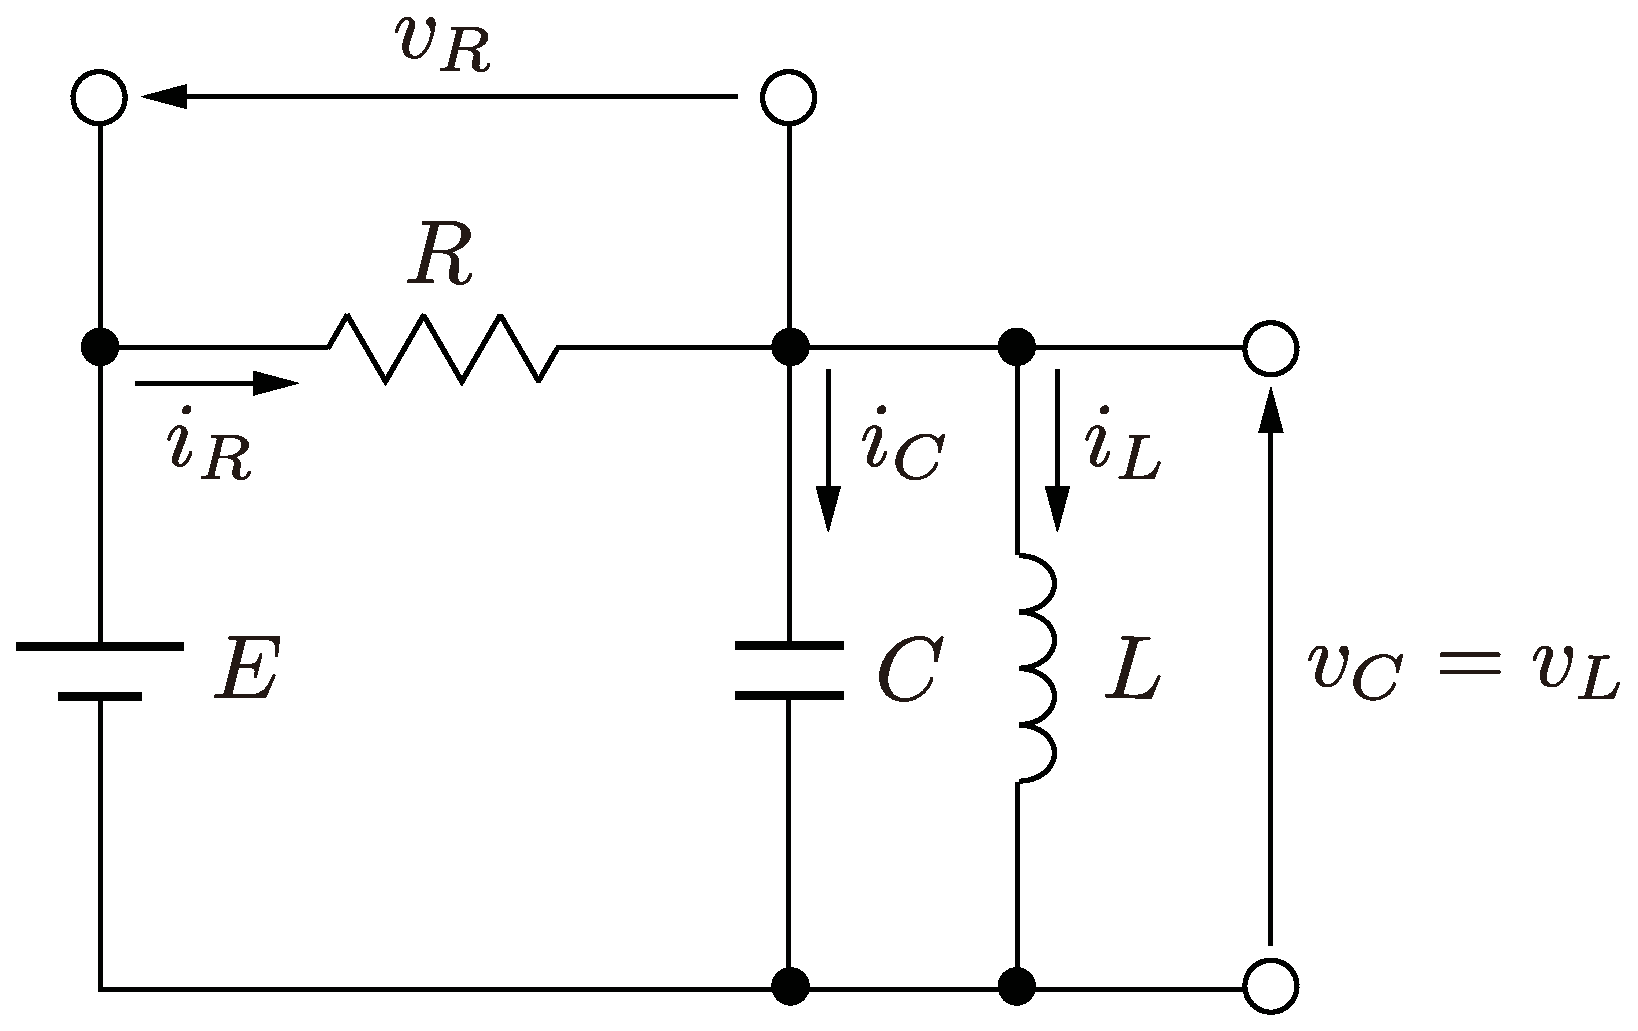
\includegraphics[width = .4\linewidth]{figs/circkawaguchi.eps}
  \medskip
  \caption{\textbf{微分代数方程式の例題:LC並列回路}}
  \label{fig:RLC}
  \medskip
\end{figure}
図\ref{fig:RLC}の簡単な電気回路において,$R=L=C=E=1$のときのシミュレーションを行うことを考える。
この回路の動的な要素はコイル$L$とコンデンサ$C$であり,その微分方程式は,
\begin{subequations}\label{eq:ex_de}
  \begin{align}
    L\dot i_L & = v_L \\
    C\dot v_C & = i_C
  \end{align}
\end{subequations}
である。ただし,初期値は$i_L(0)=0$,$v_C(0)=0$とする。
また,オームの法則とキルヒホッフの法則から,
\begin{subequations}\label{eq:ex_ae}
  \begin{align}
    v_R & =R i_R      \\
    i_R & = i_L + i_C \\
    v_L & = v_C       \\
    E   & = v_C + v_R
  \end{align}
\end{subequations}
という代数方程式が成り立つ。

このシステムは微分方程式と代数方程式が連立された
微分代数方程式である。
式\ref{eq:ex_ae}の代数方程式を用いて文字を消去すると,
等価な常微分方程式を得ることができる。
これはクロン縮約に対応し,得られる常微分方程式は,
\begin{subequations}\label{eq:ex1_ode}
  \begin{align}
    \dot{i}_L & = \frac{1}{L}v_C                     \\
    \dot{v}_C & = \frac{1}{RC}(E-v_C)-\frac{1}{C}i_L
  \end{align}
\end{subequations}
となる。まずは,この常微分方程式を解くプログラムを書いてみよう。
常備分方程式に対するMATLABのソルバとしては\verb|ode45|を用いるのが
一般的である。\verb|ode45|では,常微分方程式$\dot{x} = f(t, x)$
の関数$f(t, x)$を実装することにより常微分方程式を解くことができる。
式(\ref{eq:ex1_ode})の右辺を実装すると,プログラム\ref{program:ex1_ode}のようになる。
\begin{PROGRAMA}[count,title={func\_RLC\_ode.m}]\label{program:ex1_ode}
  \begin{verbatim}
function dx = func_RLC_ode(x, R, C, L, E)
vC = x(2);

diL = vC/L;
dvC = (E-vC)/R/C - iL/C;

dx = [diL; dvC];

end
\end{verbatim}
\end{PROGRAMA}
また,これを用いて\verb|ode45|を実行し,常微分方程式を解くプログラムは
プログラム\ref{program:main_ode1}となる。
\begin{PROGRAMA}[count,title={main\_RLC\_ode.m}]\label{program:main_ode1}
  \begin{verbatim}
R = 1;
L = 1;
C = 1;
E = 1;

func = @(t, x) func_rlc_ode(x, R, C, L, E);
x0 = [1; 1];
tspan = [0 30];

[t, x] = ode45(func, tspan, x0);
\end{verbatim}
\end{PROGRAMA}
このプログラムにおいて,出力された変数\verb|x|は,$i_L$と$v_C$の時系列を
並べたベクトルである。したがって,$i_C$や$i_R$などの他の変数については
式(\ref{eq:ex_ae})の代数方程式を用いて改めて計算する必要があることに注意しよう。

つぎに,クロン縮約を行わず,微分代数方程式を直接解くことを考える。
これには,物理的な代数方程式をそのまま用いることとができ,
複雑なシステムになっても記述が簡単である利点がある。
MATLABで微分代数方程式を解くことができるコマンドのひとつに\verb|ode15s|がある。
\verb|ode15s|は
\[
  M\dot{x} = f(x)
\]
という形で記述された微分代数方程式を対象とする。式\ref{eq:ex_de},\ref{eq:ex_ae}をこの形にあてはめると,
\[
  \begin{bmatrix}
    0 & L & 0 & 0 & 0 & 0 \\
    0 & 0 & 0 & 0 & 0 & C \\
    0 & 0 & 0 & 0 & 0 & 0 \\
    0 & 0 & 0 & 0 & 0 & 0 \\
    0 & 0 & 0 & 0 & 0 & 0 \\
    0 & 0 & 0 & 0 & 0 & 0 \\
  \end{bmatrix}
  \begin{bmatrix}
    \dot i_R \\\dot i_L\\\dot i_C\\\dot v_R\\\dot v_L\\\dot v_C
  \end{bmatrix}
  =\begin{bmatrix}
    v_L \\i_C\\v_R-R i_R\\i_R-i_L-i_C\\v_L-v_C\\E-v_C-v_R
  \end{bmatrix}
\]
となる。ここで,右辺の3番目以降の要素の順番は任意であることに注意しよう。
この右辺を実装するとプログラム\ref{program:DAE1}となる。

\begin{PROGRAMA}[count,title={func\_RLC\_DAE.m}]\label{program:DAE1}
  \begin{verbatim}
function dx = func_rlc_dae(x, R, C, L, E)

vR = x(1);
vL = x(2);
vC = x(3);
iR = x(4);
iL = x(5);
iC = x(6);

dvC = iC;
diL = vL;

con1 = vC-vL;
con2 = E-vC-vR;
con3 = iR-(iC+iL);
con4 = vR-iR*R;

dx = [dvC; diL; con1; con2; con3; con4];
end
\end{verbatim}
\end{PROGRAMA}
この関数を用いると,プログラム\ref{program:DAE1}のように微分代数方程式を解くことができる。
\begin{PROGRAMA}[count,title={main\_RLC\_DAE.m}]\label{program:DAE1}
  \begin{verbatim}
R = 1;
C = 1;
L = 1;
E = 1;

M = zeros(6, 6);
M(1, 2) = L;
M(2, 6) = C;

x0 = zeros(6, 1);
tspan = [0 30];

options = odeset('Mass', M);
func = @(t, x) func_RLC_DAE(x, R, C, L, E);
[t, y] = ode15s(func, tspan, x0, options); 
\end{verbatim}
\end{PROGRAMA}
このプログラムにおいて,10行目で初期状態をすべて0ととっているが,
意味を持つのは動的な要素の値のみ,すなわち,2番目と6番目の要素のみであり,
他の値については代数方程式を満たす値が\verb|ode15s|によって探索される。
また,解\verb|x|は,$v_R, v_L, v_C, i_R, i_L, i_C$の時系列を並べた行列であり,
常微分方程式に変換した場合と異なり,すべての物理量を含んでいる。

常微分方程式として解いた場合と微分代数方程式として解いた場合の$i_L$と$v_C$を図\ref{fig:solution_dae}
に示す。それぞれの図には\verb|ode45|と\verb|ode15s|の解の2本の線が表示してあるが,当然ながらこれらは完全に重なっている。
\begin{figure}[t]
  \centering
  {
    \begin{minipage}{0.49\linewidth}
      \centering
      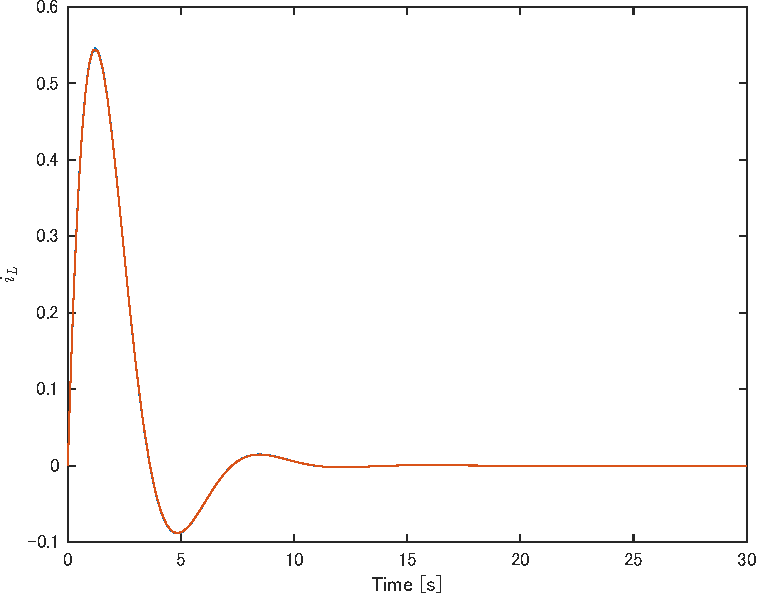
\includegraphics[width = 1.0\linewidth]{figs/i_L}
      \subcaption{$i_L$の時間応答}
    \end{minipage}
    \begin{minipage}{0.49\linewidth}
      \centering
      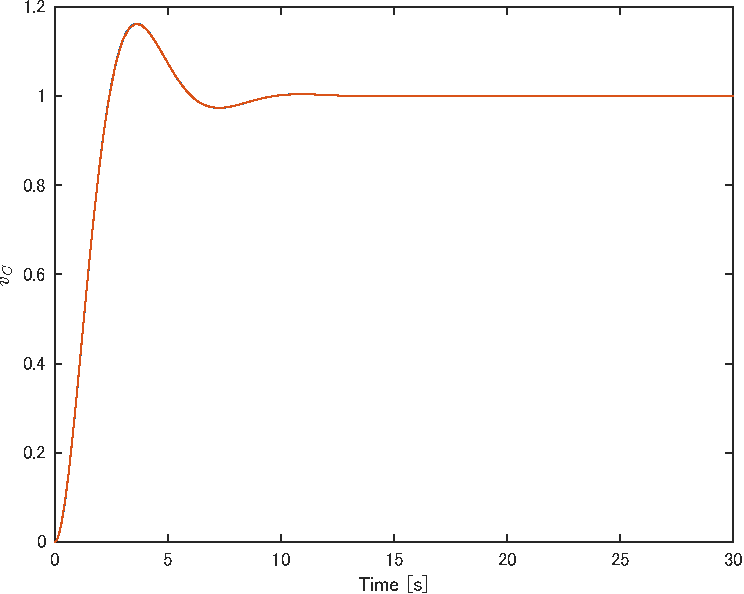
\includegraphics[width = 1.0\linewidth]{figs/v_C}
      \subcaption{ $v_C$の時間応答}
    \end{minipage}
    \medskip
    \caption{\textbf{LC並列回路の時間応答}
    }
    \label{fig:solution_dae}
  }
  \medskip
\end{figure}
\end{例}
\subsection{電力系統のシミュレーションのシンプルな実装}
本項では,電力系統のシミュレーションをシンプルに
実装する方法を説明する。
\begin{例}[電力系統のシミュレーション]\label{ex:dae_ex2}
図\ref{dummy}の電力系統のシミュレーションを行うことを考える。

\end{例}


}


\end{document}